\documentclass[conference]{IEEEtran}
\IEEEoverridecommandlockouts
% The preceding line is only needed to identify funding in the first footnote. If that is unneeded, please comment it out.
\usepackage{cite}
\usepackage{amsmath,amssymb,amsfonts}
\usepackage{algorithmic}
\usepackage{graphicx}
\usepackage{textcomp}
\usepackage{xcolor}
\graphicspath{ {./Images/} }
\def\BibTeX{{\rm B\kern-.05em{\sc i\kern-.025em b}\kern-.08em
		T\kern-.1667em\lower.7ex\hbox{E}\kern-.125emX}}
\begin{document}
	
	\title{CSC8628 Image Informatics Project}
	
	\author{\IEEEauthorblockN{Abdullah Turki H Alshadadi}
		\IEEEauthorblockA{\textit{School of Computing} \\
			\textit{Newcastle University}\\
			Newcastle upon Tyne, United Kingdom \\
			A.T.H.Alshadadi2@newcastle.ac.uk\\
			190582184}
	}		
	
	\maketitle
	
	\section{Introduction}
	This image informatics project aims to develop a classical segmentation 
	method dedicated to accurately segmenting food items within 
	the FoodSeg103 dataset. The segmentation of food holds significant 
	relevance for health-related applications, specifically in the estimation 
	of food calories and nutrients. Hence, the implementation of an accurate 
	methodology is important for achieving reliable results 
	in this context \cite{10.1145/3474085.3475201}.
	
 	\section{Algorithm Description}
 	
 	\subsection{Overview of Region Adjacency Graphs (RAGs)}
 	
 	Region Adjacency Graphs (RAGs) are a method used in image segmentation, where regions of an image are represented as nodes, and edges connect adjacent regions. My implementation is based on RAGs, leveraging the idea that neighbouring regions are likely to belong to the same object \cite{841950}\cite{868688}.

	\subsection{2.2 Image Resizing and Interpolation}
	
	To maintain consistency, I resized the images to 256x256 using the nearest neighbour interpolation method. This choice not only reduces computational power but also preserves the original colour values in the image.
 	
 	\subsection{SLIC Zero Segmentation}
 	
 	A key aspect of the algorithm involves the application of SLIC zero, a subset of the Superpixel-based Linear Index of Connectivity (SLIC) algorithm. SLIC zero's adaptive selection of the compactness parameter enables the creation of superpixels without compromising computational efficiency. These superpixels, generated through a carefully chosen segmentation method, form the basis for subsequent steps in the algorithm. The decision to use SLIC zero reflects a balance between computational efficiency and segmentation accuracy \cite{6205760}. Furthermore, in the function in  \textbf{scikit-image} I have set a Gaussian smoothing kernel to smooth the colours so that the next method could take advantage of similar colours \cite{scikit-image}.
 	
 	\subsection{RAGs Computation using Mean Colour Method}
 	The superpixels generated by SLIC zero were used to compute Region Adjacency Graphs (RAGs) using the mean colour method. This approach enhances the representation of relationships between adjacent regions by calculating the weight between two adjacent regions representing how similar two regions are in the RAGs \cite{841950}.
 	
 	\subsection{Normalised Graph Cut}
 	
 	The segmentation process culminates in the application of Normalised Graph Cut to the computed Region Adjacency Graphs. This step plays a crucial role in refining the segmentation results, ensuring the algorithm's capability to more accurately identify and delineate individual food items within the images \cite{841950}.
 	
 	\begin{figure*}[htbp]
 		\centering
 		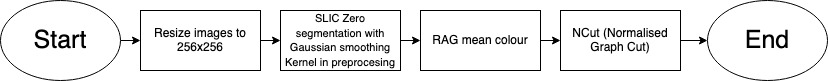
\includegraphics[width = \textwidth]{final_flowchart.jpg}
 		\caption{Flowchart of the implementation}
 		\label{fig:flowchart}
 	\end{figure*}
 	
 	\section{Libraries/Functions Used}
 	
 	\subsection{Libraries Utilized}
 	
 	The success of the algorithm is underpinned by the strategic use of various libraries:
 	
 	\begin{itemize}
 		\item \textbf{Keras}: Leveraging the \texttt{keras.utils.image\_dataset\_from\_directory()} function streamlines the process of reading and resizing the dataset \cite{chollet2015keras}.
 		
 		\item \textbf{TensorFlow}: The integration of TensorFlow is pivotal in converting the \texttt{tf.data.Dataset} to NumPy arrays using the \texttt{as\_numpy\_iterator()} method \cite{tensorflow2015-whitepaper}.
 		
 		\item \textbf{NumPy}: As a fundamental numerical library, NumPy plays a central role in representing images as arrays \cite{harris2020array}.
 		
 		\item \textbf{scikit-image}: The rich functionalities offered by scikit-image are harnessed for various image processing tasks \cite{scikit-image}.
 		
 		\item \textbf{Matplotlib}: Serving as a versatile plotting library, Matplotlib aids in visually presenting images and critical figures \cite{Hunter:2007}.
 	\end{itemize}
 	
 	\section{Results Presentation}
 	
 	\begin{figure}[htbp]
 		\centerline{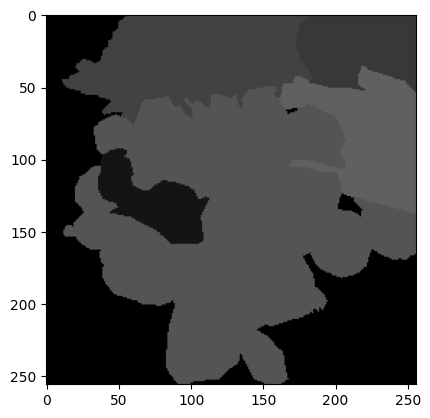
\includegraphics[width = 0.4\textwidth]{groundtruth.png}}
 		\caption{\texttt{00000048.jpg} Ground truth image}
 		\label{fig:groundtruth}
 	\end{figure}
 	
 	 \begin{figure}[htbp]
 		\centerline{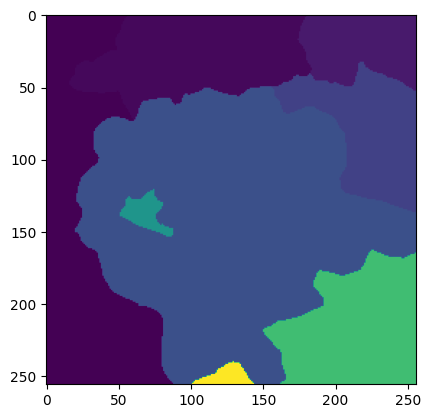
\includegraphics[width = 0.4\textwidth]{label.png}}

 		\caption{\texttt{00000048.jpg} My own implementation results}
 		\label{fig:segmented}
 	\end{figure}
 	
 	 \begin{figure}[htbp]
 		\centerline{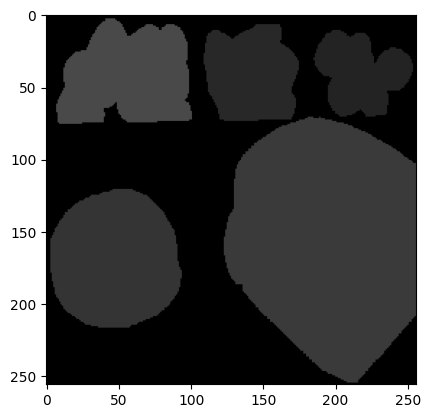
\includegraphics[width = 0.4\textwidth]{bad-ground-truth.png}}
 		\caption{ \texttt{00001977.jpg} My own implementation results}
 		\label{fig:badgroundtruth}
 	\end{figure}
 	
 	\begin{figure}[htbp]
 		\centerline{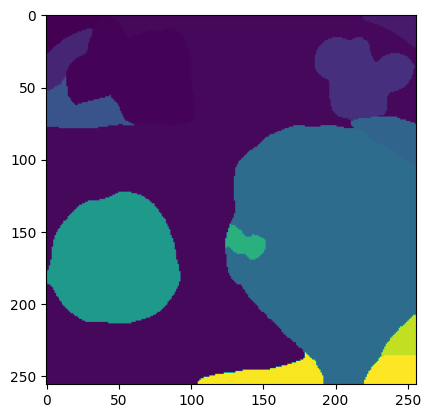
\includegraphics[width = 0.4\textwidth]{badlabel.png}}
 		\caption{\texttt{00001977.jpg}  My own implementation results}
 		\label{fig:badsegmented}
 	\end{figure}
 	
 	
 	
 	\subsection{Dataset Overview}
 	
 	The examination of a specific image, \texttt{00000048.jpg} Fig.\ref{fig:groundtruth}, from the dataset serves as a testament to the algorithm's proficiency in accurately segmenting food items. However, a nuanced limitation emerges in the absence of a background mask. This absence leads to the segmentation of the background into sections, even when the background shares the same colour. This nuanced challenge prompts a closer look at background segmentation intricacies.
 	
 	\subsection{Challenges in Background Masking}
 	
 	Background masking proves to be a formidable challenge due to the diverse colour schemes inherent in different images. For instance, the image \texttt{00001977.jpg} Fig.\ref{fig:extra_vis2} presents a scenario where a green plate sits on a white table, adding complexity to the masking process. The presence of shadows further exacerbates the difficulty in achieving accurate background removal. These challenges underscore the need for robust methods capable of overcoming the intricacies of background masking in diverse and dynamic scenarios.
 	
 	\section{Key Findings and Discussions}
 	
 	\subsection{Strengths and Limitations}
 	
 	The algorithm showcases its strengths in effectively segmenting food items, as demonstrated by the successful segmentation of image \texttt{00000048.jpg} Fig.\ref{fig:segmented}. However, the absence of a background mask introduces challenges, leading to the unnecessary segmentation of the background particularly when the food extends into the background. This limitation accentuates the necessity for continued refinement in background removal techniques to enhance the overall accuracy of the segmentation algorithm.
 	
 	\subsection{Future Considerations}
 	
 	Looking ahead, future endeavours will concentrate on the development of an adaptive masking method. This aims to address the identified limitations by enhancing background removal. The objective is to enable the segmentation algorithm to focus on isolating food items without unnecessary interference from the background. This future trajectory holds promise for significant improvements in the algorithm's overall performance and accuracy.
 	
 	\section{Conclusions}
 	
	In summary, the implemented algorithm demonstrates proficiency in segmenting food items but encounters challenges in background segmentation, particularly with varying colours and shadows. Future endeavours will focus on developing an adaptive masking method to address this limitation. The aim is to create a masking approach that dynamically removes background interference, allowing the segmentation algorithm to focus on accurately identifying and segmenting food items without unnecessary divisions caused by the background.


	\bibliographystyle{IEEEtran}
	\bibliography{bibliography.bib}
	
	\newpage
	
	\section*{Appendix}
	
	 \begin{figure}[htbp]
		\centerline{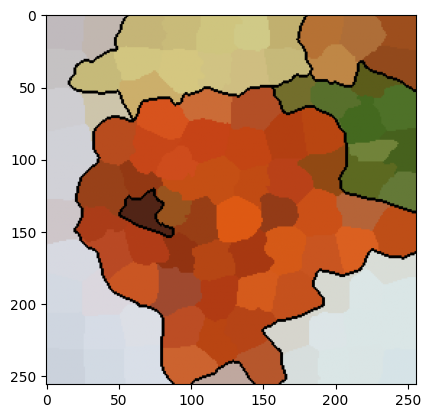
\includegraphics[width = 0.4\textwidth]{slic.png}}
		\centerline{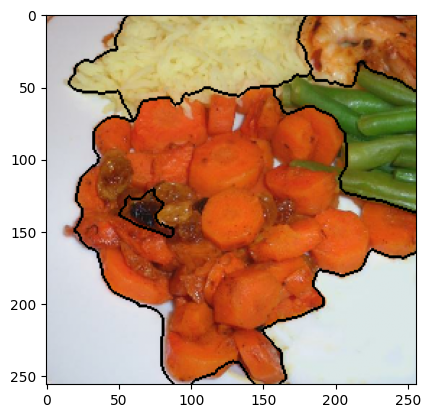
\includegraphics[width = 0.4\textwidth]{sliconreal.png}}
		\caption{\texttt{00000048.jpg} Further visualisation of my implementation results}
		\label{fig:extra_vis}
	\end{figure}
	
	
	\begin{figure}[htbp]
		\centerline{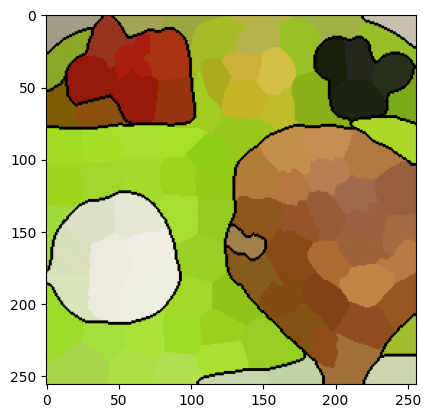
\includegraphics[width = 0.4\textwidth]{badslic.png}}
		\centerline{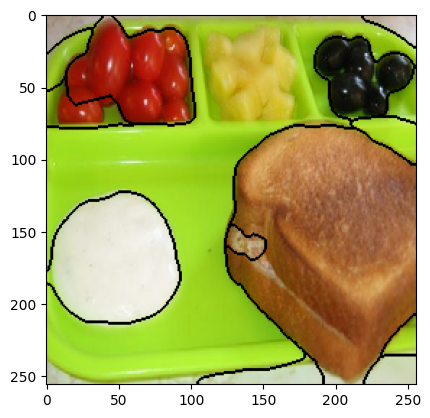
\includegraphics[width = 0.4\textwidth]{badbackground.png}}
		\caption{\texttt{00000048.jpg} Further visualisation of my implementation results}
		\label{fig:extra_vis2}
	\end{figure}
	
	
\end{document}
